% UFO camera user manual 
%

\chapter{Operation manual}

\section{Concept}

A high performance camera interface combined with application specific camera controllers opens 
a wide range of opportunities for scientific applications. Figure \ref{camera-setup} shows the first 
prototype of the fully programmable high-throughput UFO camera currently developed at KIT. 

The main features of the UFO camera are:

\begin{itemize}
\item Modular concept with fast FMC interface between camera controller and image sensor. With minimal effort a large variety of image sensors can be included in the setup.
\item Powerful high bandwidth firmware to handle data rate currently up to 2GByte/sec.
\item Fast interface to the readout PC using a PCI Express extender. High performance Linux drivers for the architecture are available.
\item Interfaces for attaching application specific logic in FPGA and driver.
\end{itemize}

\begin{figure}
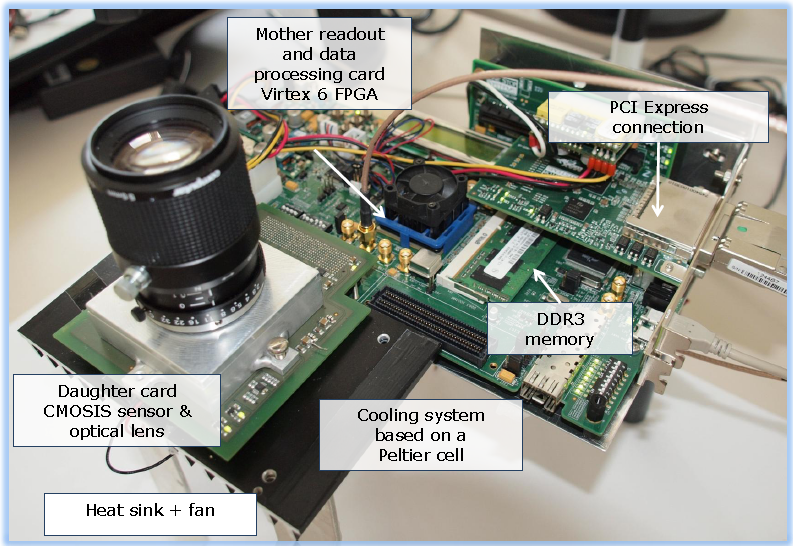
\includegraphics[width=\textwidth]{images/Figure_2.png}
\caption{\label{camera-setup} Prototype of the modular UFO camera.}
\end{figure}




\section{Supported image sensors}

The prototype of the UFO camera has been developed using the images sensor CMOSIS CMV2000 with 2.2 mega pixel and frames rates of up to 340 fps in full resolution. The sensor supports to modes of operation with 10bit and 12bit resolution \cite{CMOSIS:CMV2000}. 

A full list of supported and future sensors is given in table \ref{image-sensors}.



\begin{table}
\caption{\label{image-sensors} List of supported image sensors.}
\begin{center}
\begin{tabular}{|c|c|p{8cm}|}
\hline
Image sensor 			&  Mode 		& Comment \\
\hline
CMOSIS CMV2000 		& 10bit, 340fps & Implemented, tested, characterized \\
\hline
CMOSIS CMV2000		& 12bit, 70fps	& Implemented, tested, characterized \\
\hline
CMOSIS CVM4000		& 			& Ordered. Note: the sensor is pin compatible with the smaller CMV2000 and provides the same operation mode \cite{CMOSIS:CMV4000}. \\
\hline
Fairchild CIS1021		& 2x11bit, 100fps & Planned \cite{FAIRCHILD:CIS1021}\\
\hline
\end{tabular}
\end{center}
\end{table}


\section{Starting the camera}
Camera and readout PC are considered as a unit. In order to establish word with the camera 
prototype a certain procedure has to be followed.

\begin{itemize}
\item First, the camera has to be turned ON while the readout PC is ON.
\item Reboot the readout PC. Currently only then the connection is properly established.
\item Check that the camera is operational. 

The LEDs on the controller board should show the following values:\\
DS19 blinking, DS18 ON, DS20  ON, DS17 OFF. 

All three LEDs on FMC board should be ON to indicate proper voltage levels.

CBL and EDGE LEDs should be ON to indicate proper PCIe connection. 
\item Select the desired frame rate using the script \verb/Reset_<bitrate>_bits.sh/
\item Check again the status. 

Now also the LEDS DS21, DS14, DS15 need to be ON.
\end{itemize}


\subsection{LED status indicators}

For visual confirmation of the camera's proper working state, number of LED indicators are provided on the camera controller board, shown in \figurename~\ref{pic_LED}. The description of this LEDs is given in \tablename~\ref{LEDs}. 

For other existing LEDs on the FPGA main board, they are related to ML605 board functionality \cite{XILINX:ML605}.
Beside the visual information of the LEDs more details are given by the status register of the camera. 

\begin{figure}[p]
\centering
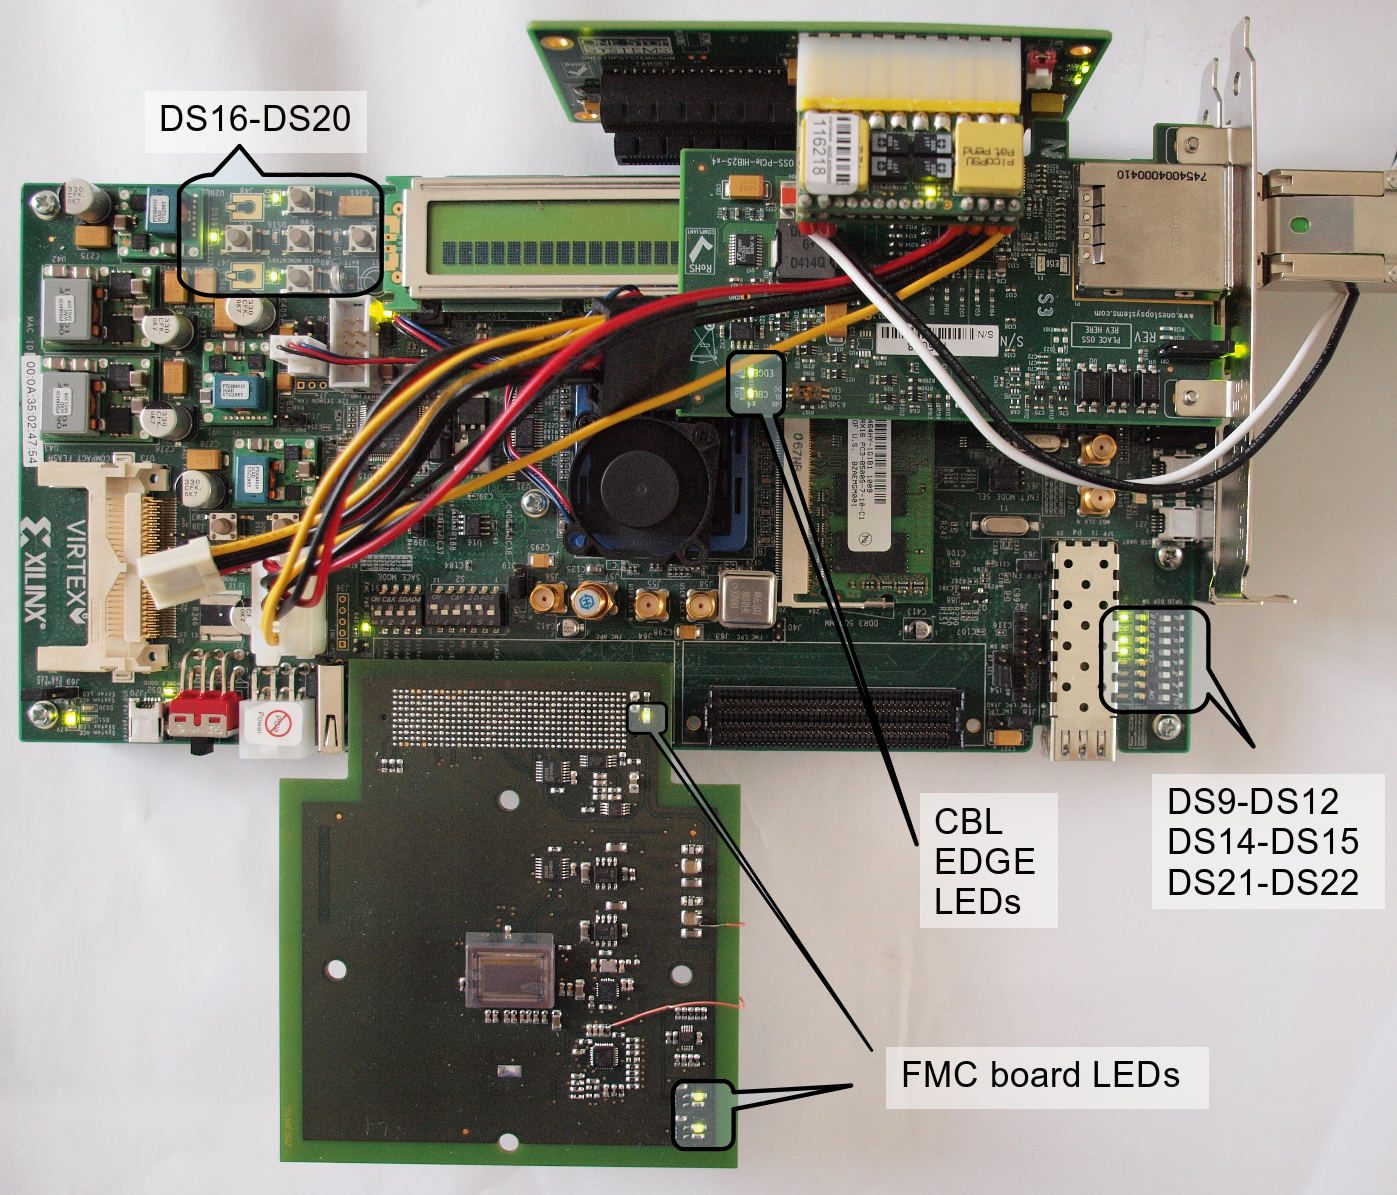
\includegraphics[width=0.7\textwidth]{images/pic_LEDs.png}
\caption{\label{pic_LED} Camera indicator LEDs}
\end{figure}


\begin{table}[p]
\caption{\label{LEDs} List of status LEDs on the camera controller board.}
\begin{center}
\begin{tabular}{|c|c|c|}
\hline
LED					& Status 		& Comment \\
\hline
DS18 				& On			&  DDR3 initialization has completed \\
\hline
DS16				& On			& Readout in progress \\
\hline
DS14				& On			& data register is locked\\
\hline
					& Off, Flashing	& data register doesn’t work correctly \\
\hline
DS15				& On			& status register is locked\\
\hline
					& Off, Flashing	& status register doesn’t work correctly \\
\hline
DS19				& Flashing	& 200 MHz clock is alive \\
\hline
DS21				& On			& Busy active \\
\hline
DS17				& Off			& PCIe connection is properly established \\
\hline
DS12				& On			& DMA ready to accept data \\

\hline
\end{tabular}
\end{center}
\end{table}


\newpage
\subsection{Reset scripts}
The script \verb/Reset_<bitrate>_bits.sh/ will report if initialization completed successfully. 
If initialization is executed successfully the status  OK  is printed and the camera is ready for operation.

Example: configuring camera for 12 bit mode  

\begin{lstlisting}
ufo@ufocamera:~> Reset_Init_all_reg_12bit.sh
 Reset Readout and CMOSIS 
 Release Reset for Readout
 Start CMOSIS Configuration ..
 12 - bit mode, set Bit_mode 
 12 bit mode, set ADC resolution 12 bits 
 End CMOSIS Configuration ..
 Write exp time......
 cmosis_number_lines = 1088
 Camera READY ........ OK
\end{lstlisting}


\newpage
\section{Camera interfaces}

The camera can be used by a graphical user interface. It displays life images and provides access to all camera parameters. 
For automation of purpose the powerful command-line tool pcitool is available. The distribution contains several scripts that 
implement some often used functions.

\subsection{Graphical camera user interface}

The camera comes with a graphical application that displays live images from the camera. 
The bottom tab provides some short cuts for often used camera functions. 
The full set of camera properties are accessible in the right part of the application. 

The graphical user inferface is shown in \figurename~\ref{camera-gui}.  The main screen display the image data from the camera. The control buttons above the main window allow an video recorder like recording and replay of the selected scenes.
The bottom part provides some shortcuts for often used camera parameters.  The full set of camera properties are accessible in the right part of the application. With the double click on the parameter name the value can be changed. All sensor registers are accessible as well. 

\begin{figure}[h]
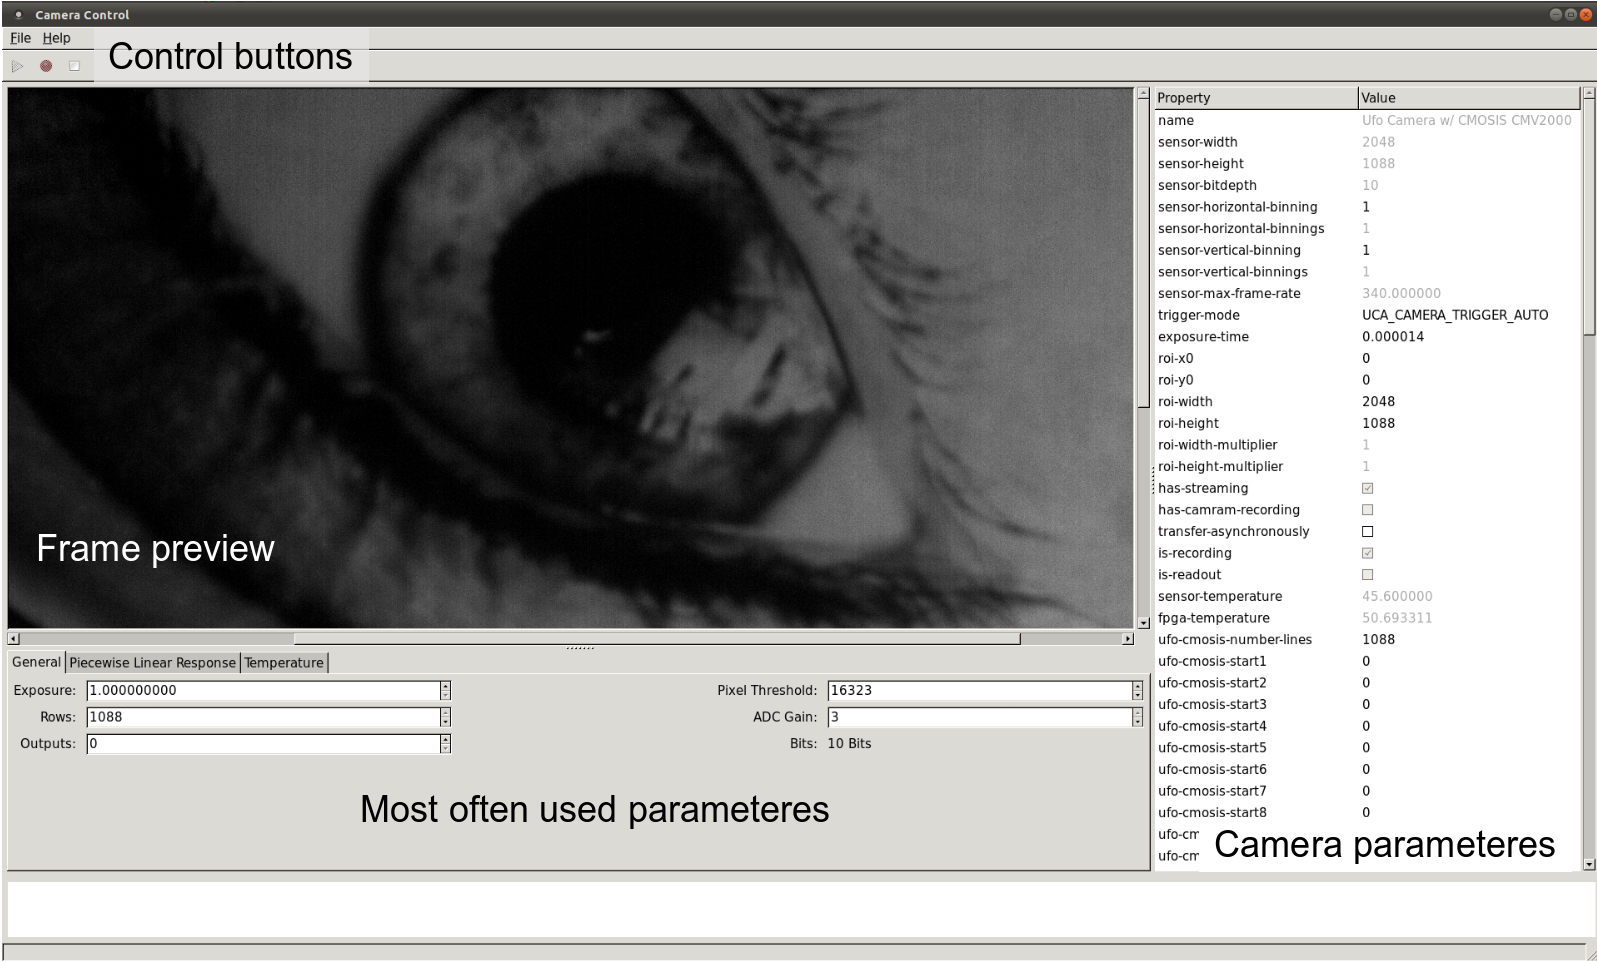
\includegraphics[width=\textwidth]{images/ufo_gui2.png}
\caption{\label{camera-gui} Camera frontend}
\end{figure}


\subsubsection{Set camera parameters}

Select the parameter "Exposure" in the bottom window, increment the value, or directly writing the desired value in the appropriate space. The value should be given in units of seconds. Alternatively the parameter "exposure-time" from the  parameter list in the right window could be chosen.

\subsubsection{Piecewise-linear response function}

The camera can be used with a piecewise linear response function. This gives the possibility to achieve a virtual higher optical dynamic range. The feature will clip illuminated pixels which reach a programmable voltage, while leaving the darker pixels untouched. The clipping level can be adjusted 2 times within one exposure time to achieve a maximum of 3 slopes in the response curve. In the dislay it is shown using bar for piecewise linear response. It is shown in  \figurename~\ref{ufo_gui_piecewise_bar}. 

More information for using the piecewise can be found in CMOSIS2000 reference sheet \cite{CMOSIS:CMV2000}.

\begin{figure}[h]
\centering
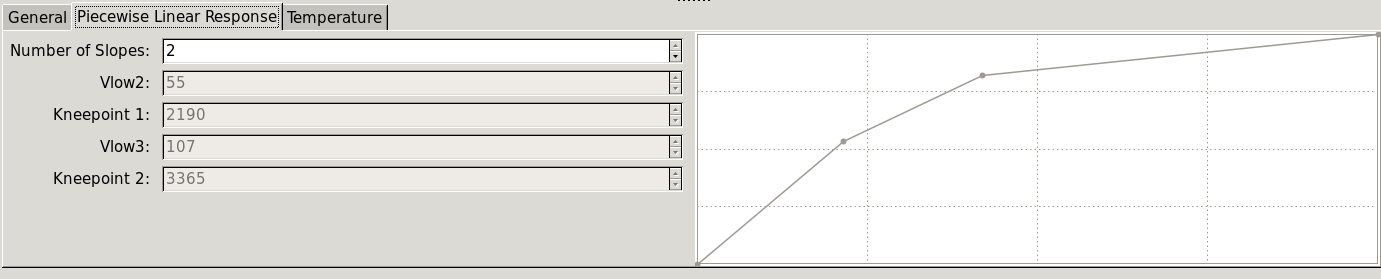
\includegraphics[width=1\textwidth]{images/ufo_gui_piecewise_bar.png}
\caption{\label{ufo_gui_piecewise_bar} Dialog to customize the piecewise linear response function}
\end{figure}

\subsubsection{Monitoring of the camera temperatures}

Finally the temperature of sensor and FPGA is monitored. It is shown in  \figurename~\ref{ufo_gui_temp_bar}. Alarm would indicate if the temperature of the FPGA exceeds the alarm limits. 
\begin{figure}[h]
\centering
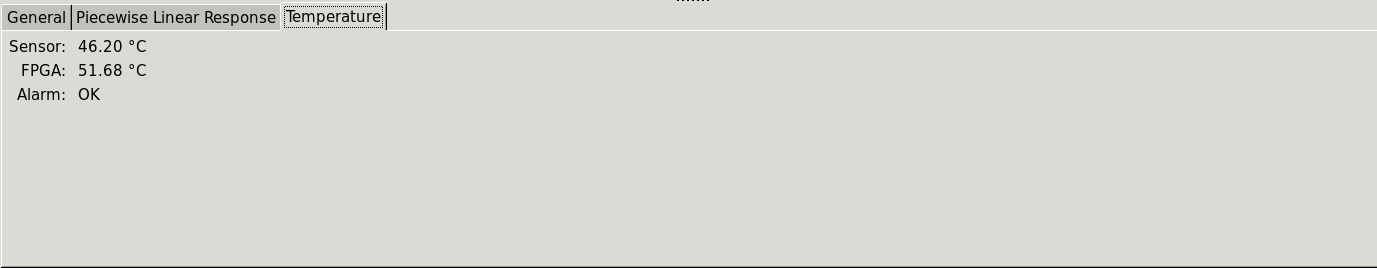
\includegraphics[width=\textwidth]{images/ufo_gui_temp.png}
\caption{\label{ufo_gui_temp_bar} Sensor temperature monitoring}
\end{figure}



%TODO: How to save a picture with the GUI?


% Host: ipecamera

\subsection{Command line tools in pci-tools}



The pcitools provide complete control of all camera properties. It allows to read and write the camera registers,
trigger frame acquisition, initiate DMA transfers, and check the status of active operations. Basically, the command is
executed as follows:

\begin{verbatim}
pci <mode> [options] [hex data]
\end{verbatim}

The first argument mode defines the global mode of operation. Examples are retrieving current camera configuration, 
reading and writing registers and device memory, performing DMA transfers, or performing continuous frame grabbing.  
There mode of operation is followed by one or more options that specify various parameters like the register name or address to read/write, required frame rate, number of frames to grab, etc. Finally, the hex data is hex 
decimal values written to the registers. More information about of the pcitool usage can be found 
with \verb/pci -h/. 

\begin{lstlisting}
ufo@ufocamera:~> pci -h
Usage:
 pci <mode> [options] [hex data]
  Modes:
   -i				- Device Info
   -l[l]			- List (detailed) Data Banks & Registers
   -r <addr|reg|dmaX>		- Read Data/Register
   -w <addr|reg|dmaX>		- Write Data/Register
   --benchmark <barX|dmaX>	- Performance Evaluation
   --reset			- Reset board
   --help			- Help message

  Event Modes:
   --trigger [event]		- Trigger Events
   -g [event]			- Grab Events

  DMA Modes:
   --start-dma <num>[r|w]	- Start specified DMA engine
   --stop-dma [num[r|w]]	- Stop specified engine or DMA subsystem
   --list-dma-engines		- List active DMA engines
   --list-dma-buffers <dma>	- List buffers for specified DMA engine
   --read-dma-buffer <dma:buf>	- Read the specified buffer
   --wait-irq <source>		- Wait for IRQ

  Kernel Modes:
   --list-kernel-memory 	- List kernel buffers
   --read-kernel-memory <blk>	- Read the specified block of the kernel memory
				  block is specified as: use:block_number
   --free-kernel-memory <use>	- Cleans lost kernel space buffers (DANGEROUS)
	dma			- Remove all buffers allocated by DMA subsystem
	#number			- Remove all buffers with the specified use id

  Addressing:
   -d <device>			- FPGA device (/dev/fpga0)
   -m <model>			- Memory model (autodetected)
	pci			- Plain
	ipecamera		- IPE Camera
   -b <bank>			- PCI bar, Register bank, or DMA channel

  Options:
   -s <size>			- Number of words (default: 1)
   -a [fifo|dma]<bits>		- Access type and bits per word (default: 32)
   -e <l|b>			- Endianess Little/Big (default: host)
   -o <file>			- Append output to file (default: stdout)
   -t <timeout|unlimited> 	- Timeout in microseconds

  Event Options:
   --event <evt>		- Specifies event for trigger and grab modes
   --data <type>		- Data type to request for the events
   --run-time <us>		- Limit time to grab/trigger events
   -t <timeout|unlimited>	- Timeout to stop if no events triggered
   --trigger-rate <tps>		- Generate tps triggers per second
   --trigger-time <us>		- Specifies delay between triggers (us)
   -s <num|unlimited> 		- Number of events to grab and trigger
   --format [type]		- Specifies how event data should be stored
	raw			- Just write all events sequentially
	add_header		- Prefix events with 512 bit header:
				  event(64), data(64), nope(64), size(64)
				  seqnum(64), offset(64), timestamp(128)
   --buffer [size]		- Request data buffering, size in MB
   --threads [num]		- Allow multithreaded processing

  DMA Options:
   --multipacket		- Read multiple packets
   --wait			- Wait until data arrives

  Information:
   --verbose [level]		- Announce details of ongoing operations
   -q				- Quiete mode (suppress warnings)

  Data:
	Data can be specified as sequence of hexdecimal number or
	a single value prefixed with '*'. In this case it will be
	replicated the specified amount of times
	
\end{lstlisting}


Example: read the exposure time

\begin{verbatim}
pci -r cmosis_exp_time
\end{verbatim}

\begin{description}
\item[] The argument  \verb/-r cmosis_exp_time/ reads the register from the image sensor. 
\end{description}




\section{Working with the camera}

This section describes common operations with the pcitools. 


\subsection{Take a single picture}

\begin{verbatim}
pci --grab -s 1 --trigger -o <output_image>
\end{verbatim}

\begin{description}
\item[ ] Mode \verb/--grab/ instructs pcitool to start grabbing
\item[ ] \verb/-s 1/ option specifies that only a single frame is required
\item[ ] \verb/--trigger/ instructs camera to self trigger, if this option not provided the pcitool will wait
until camera will decide to send the frame (possibly triggered by external hardware trigger)
\item[ ] \verb/-o <output_image>/ specifies the file to store images. The images are stored in raw format, each 16 bit word describing a single pixel. The horizontal dimension is changing before vertical.
\end{description}

The raw image data does not contain information on image size and colors. This information has to be specified when the image should be displayed. Standard image analysis applications like \emph{Imagej} \cite{SW:IMAGEJ} have raw data import filter that allow to decode the data correctly. 
The following examples shows the import dialog of an ImageJ distribution called \emph{Fiji} \cite{SW:FIJI}. 

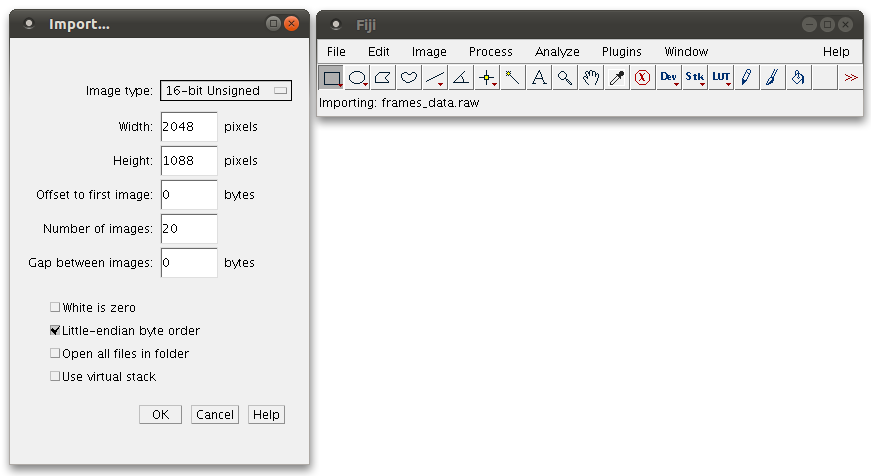
\includegraphics[width=\textwidth]{images/Fiji_set_param.png}

For opening the frame(s) we should execute: \textbf{File} $\rightarrow $ \textbf{Import} $ \rightarrow $ \textbf{Raw...}. After the selection of the frame we should set the frame info: width, height, it's size, endianess, and number of frames. When hovering over the picture with the mouse, in the status bar of the \emph{Fiji} is shown the pixel position and pixel value. In the upper left corner of the picture are additional informations: which frame is displayed, how many frames are open, size of the frame, etc.




\subsection{Taking a series of pictures}
Similarly, multiple images may be grabbed

\begin{verbatim}
pci --grab --run-time <us> --trigger --trigger-rate <fps> -o <output_image>
\end{verbatim}

In this case:
\begin{description}
\item[ ] \verb/--run-time <us>/ option specifies how long to grab frames in microseconds
\item[ ] \verb/--trigger-rate <fps>/ option instructs pcitool how often to issue software triggers. This value is desired frame rate in frames per second
\item[ ] \verb/-o <output_image>/ option agains specifies the output file. The frames are stored sequentially one after another in a single file
\end{description}

There is additional options which may define the duration and speed of grabbing process
\begin{description}
\item[ ] \verb/--trigger-time <time>/ is alternative way to define the frame rate. In this case, the interval between triggers in microseconds is specified.
\item[ ] \verb/-s <num>/ limits the number of frames to grab. It is possible to specify both \verb/--run-time/ and \verb/-s/. In this case the grabbing will terminate on each of conditions.
\item[ ] \verb/-s unlimited/ requires camera to grab infinitely or until \verb/Ctrl+C/ is pressed.
\item[ ] \verb/-t <timeout>/ instructs camera to stop grabbing if new frames are not triggered within the specified timeout (in microseconds).
\end{description}


The image file now contains a series of images in 16bit raw format. The sequence can be displayed by \emph{Fiji} as shown for the single frame case above.



\subsection{Exploring camera parameters}

The camera parameters, like exposure time, are set to optimal defaults by the initialization script. During camera operation it is possible to adjust this parameters as needed using camera registers. To get the list of all registered registers along with current values, call:
\begin{verbatim}
pci -r 
\end{verbatim}
The read command will read by default all known registers.


The detailed description of the registers may be obtained with
\begin{verbatim}
pci -l
\end{verbatim}

\begin{lstlisting}
ufo@ufocamera:~> pci -l
 BAR 0 - MEM32, Start: 0xf7ff0000, Length: 0x   10000, Flags: 0x00040200
 BAR 1 - MEM32, Start: 0xf7fee000, Length: 0x    2000, Flags: 0x00040200
 BAR 2 - MEM32, Start: 0xf7fec000, Length: 0x    2000, Flags: 0x00040200

DMA Engines: 

Banks: 
 0x00 cmosis: CMOSIS CMV2000 Registers
 0x01 fpga: IPECamera Registers
 0x80 dma: DMA Registers

Registers: 
 0x01 (16 RW) cmosis_number_lines
 0x03 (16 RW) cmosis_start1
 0x05 (16 RW) cmosis_start2
 0x07 (16 RW) cmosis_start3
 0x09 (16 RW) cmosis_start4
 0x0b (16 RW) cmosis_start5
 0x0d (16 RW) cmosis_start6
 0x0f (16 RW) cmosis_start7
 0x11 (16 RW) cmosis_start8
 0x13 (16 RW) cmosis_number_lines1
 0x15 (16 RW) cmosis_number_lines2
 0x17 (16 RW) cmosis_number_lines3
 0x19 (16 RW) cmosis_number_lines4
 0x1b (16 RW) cmosis_number_lines5
 0x1d (16 RW) cmosis_number_lines6
 0x1f (16 RW) cmosis_number_lines7
 0x21 (16 RW) cmosis_number_lines8
 0x23 (16 RW) cmosis_sub_s
 0x25 (16 RW) cmosis_sub_a
 0x27 ( 1 RW) cmosis_color
 0x28 ( 2 RW) cmosis_image_flipping
 0x29 ( 2 RW) cmosis_exp_flags
 0x2a (24 RW) cmosis_exp_time
 0x2d (24 RW) cmosis_exp_step
 0x30 (24 RW) cmosis_exp_kp1
 0x33 (24 RW) cmosis_exp_kp2
 0x36 ( 2 RW) cmosis_nr_slopes
 0x37 ( 8 RW) cmosis_exp_seq
 0x38 (24 RW) cmosis_exp_time2
 0x3b (24 RW) cmosis_exp_step2
 0x44 ( 2 RW) cmosis_nr_slopes2
 0x45 ( 8 RW) cmosis_exp_seq2
 0x46 (16 RW) cmosis_number_frames
 0x48 ( 2 RW) cmosis_output_mode
 0x4e (12 RW) cmosis_training_pattern
 0x50 (18 RW) cmosis_channel_en
 0x52 ( 3 RW) cmosis_special_82
 0x59 ( 8 RW) cmosis_vlow2
 0x5a ( 8 RW) cmosis_vlow3
 0x64 (14 RW) cmosis_offset
 0x66 ( 2 RW) cmosis_pga
 0x67 ( 8 RW) cmosis_adc_gain
 0x6f ( 1 RW) cmosis_bit_mode
 0x70 ( 2 RW) cmosis_adc_resolution
 0x73 ( 1 RW) cmosis_special_115
 0x00 (32 RW) spi_conf_input
 0x10 (32 R ) spi_conf_output
 0x20 (32 RW) spi_clk_speed
 0x30 (32 R ) firmware_info
 0x40 (32 RW) control
 0x50 (32 R ) status
 0x54 (32 R ) status2
 0x58 (32 R ) status3
 0x5c (32 R ) fr_status
 0x70 (32 R ) start_address
 0x74 (32 R ) end_address
 0x78 (32 R ) rd_address
 0xa0 (32 R ) fr_param1
 0xb0 (32 RW) fr_param2
 0xc0 (32 R ) skiped_lines
 0x100 (32 RW) rawdata_pkt_addr
 0x110 (32 R ) temperature_info
 0x120 (32 R ) num_lines
 0x130 (32 R ) start_line
 0x140 (32 R ) exp_time
 0x150 (32 RW) motor
 0x160 (32 R ) write_status
 0x170 (32 RW) num_triggers
 0x180 (32 RW) trigger_period
 0x190 (32 R ) temperature_sample_period
 0x1a0 (32 RW) max_frames
 0x1b0 (32 R ) num_frames
 0x4000 (32 RW) dma_control_and_status
 0x8000 (32 R ) dma_design_version
 0x8200 (32 R ) dma_transmit_utilization
 0x8204 (32 R ) dma_receive_utilization
 0x8208 (32 R ) dma_mwr
 0x820c (32 R ) dma_cpld
 0x8210 (12 R ) dma_init_fc_cpld
 0x8214 ( 8 R ) dma_init_fc_cplh
 0x8218 (12 R ) dma_init_fc_npd
 0x821c ( 8 R ) dma_init_fc_nph
 0x8220 (12 R ) dma_init_fc_pd
 0x8224 ( 8 R ) dma_init_fc_ph

Events: 
 new_frame
    image: 16 bit pixel data
    raw: raw data from camera
    cmask: change mask

\end{lstlisting}

In order to include the sub-registers (bit fields) into the output call
\begin{verbatim}
pci -ll
\end{verbatim}

Example: Read and adjust the exposure time

The value of single register may be read with:
\begin{verbatim}
pci -r cmosis_exp_time
\end{verbatim}

The following command will modify a register:
\begin{verbatim}
pci -w cmosis_exp_time 0x25
\end{verbatim}



\subsection{Standard scripts}

For often used operations pcitool contains scripts.
The scripts are self-explanatory. More information, if needed, can be found inside the scripts itself.

\begin{tabular}{|c|p{10cm}|}
\hline
Script						& Description \\
\hline
\verb/Status.sh/			& For reading the status of the bank register. Field description is provided in accompanying spreadsheet file. \\
\hline
\verb/Reset_10_bits.sh/ 	& Reset sequence for setup with the 10bit/pixel. \\
\hline

\verb/Reset\_11\_bits.sh/ 	& Reset sequence for setup with the 11bit/pixel. \\
\hline
\verb/Reset\_12\_bits.sh/ 	& Reset sequence for setup with the 12bit/pixel. \\
\hline
\verb/frame.sh/ 			& For requesting frames. Number of frames and exposure time is settable by user. \\
\verb/stimuli.sh/			& \\
\hline
\end{tabular}

% TODO: Display the status output and describe?!


%\subsection{Performing calibration of the image sensor}

% TODO: Add description of scripts used to calibrate the sensor



\section{Advanced options of pcitool}

\subsection{Using DMA engine and accessing raw data}

UFO Camera uses the DMA engine to deliver frames at high rate. Pcitool provides direct access to the DMA engine and allows complex scripting to perform conditional grabbing or debug the camera problems. To achieve this pcitool's DMA engine supports two modes of operation: normal and persistent. In normal mode, the DMA engine is started at each invocation of pci command and is stopped before the application termination. It suits perfectly well the standard grabbing applications. However, it is not enough if complex procedure have to be scripted. In this case, the user should start DMA engine with following command:
\begin{verbatim}
pci --start-dma <dma_engine_id>
\end{verbatim}

The DMA engine will stay running after command termination and may be verified with 
\begin{verbatim}
pci --list-dma-engines
\end{verbatim}
command. Then, multiple camera operations may be executed. The DMA engine will stay running through these operations. The small buffer will be allocated in the kernel memory space and will accept data coming from camera. When data required, the user will query DMA engine and currently buffered data will be immediately available for further processing. 

To give an example, the following alternative procedure may be used to grab frames directly using DMA engine. First DMA engine for reading from using the first DMA channel should be started
\begin{verbatim}
pci --start-dma dma1r
\end{verbatim}

The new frame may be triggered with following commands:
\begin{verbatim}
pci -w control 1e9
usleep 100000
pci -w control 1e1
pci -w control 3e1
\end{verbatim}
The first command sends frame request to control register. Then, the script pauses until camera recognizes request and third command cleans the frame request bit from the control register. Finally, the last command enables readout.

Afterwards, the camera will deliver the data to the described kernel buffers. To read the data, the following command may be executed:
\begin{verbatim}
pci -r dma1 --multipacket -o <image file>
\end{verbatim}

\begin{description}
\item[ ] Mode \verb/-r dma1/ indicates that we want to read from DMA-engine \verb/dma1/.
\item[ ] DMA option \verb/--multipacket/ indicates that we want to read all DMA engine buffers, otherwise only one buffer (4KB)[check the size of the buffer] would be read out.
\item[ ] \verb/-o/ option again specifies image file where to store results.
\end{description}

Finally, the DMA engine must be stopped if we don't want to grab further frames. The following command will do it
\begin{verbatim}
pci --stop-dma
\end{verbatim}


However, directly from DMA the data will be returned in internal format of UFO camera, not a pixel data. To decode the format and get actual image, the \verb/ipedec/ command from ufodecode package is required.

To see which parameters could \verb/ipedec/ have, type following in console:
\begin{lstlisting}
ufo@ufocamera:~> ipedec -h
usage: ipedec [OPTION]... FILE [FILE ...]
Options:
  -h, --help                Show this help message and exit
  -v, --verbose             Print additional information on STDOUT
  -r, --num-rows=N          N rows that are contained in the file
  -c, --clear-frame         Clear the frame for each iteration
  -d, --dry-run             Do not save the frames
  -f, --print-frame-rate    Print frame rate on STDOUT
      --print-num-rows      Print number of rows on STDOUT
\end{lstlisting}

The command 
\begin{verbatim}
ipedec <image file>
\end{verbatim}
creates the decoded file \verb/<image file>.raw/. The application supports one or more frames in the file. It is also possible to grab multiple frames using standard approach in the UFO camera native format. To achieve this, \verb/--format/ option may be added to standard grab command:
\begin{verbatim}
pci --grab --run-time --trigger --trigger-rate 30 -o <output_image> --format raw
\end{verbatim}


\subsection{Direct access to the PCI register space}

The bank register is implemented in BAR0 address space. It address is BAR0 address + 0x9000. 

The addresses of pci bar are reported by 
\begin{verbatim}
ufo@ufocamera:~> pci -i
Vendor: 10ee, Device: 6081, Interrupt Pin: 1, Interrupt Line: 11
BAR 0 - MEM32, Start: 0xfe400000, Length: 0x   10000, Flags: 0x00040200
BAR 1 - MEM32, Start: 0xfe412000, Length: 0x    2000, Flags: 0x00040200
BAR 2 - MEM32, Start: 0xfe410000, Length: 0x    2000, Flags: 0x00040200
\end{verbatim}

Now it is possible to read with \verb/pci -r 0xfe409000 -s 32/ the first 32 bytes of the BAR0 starting with offset 0x9000 (the actual location of UFO camera registers):
\begin{verbatim}
ufo@ufocamera:~> pci -r 0xfe409000 -s 32
fe409000:  00003200  00000000    00003200  00000000
fe409010:  000b3200  00000000    000b3200  00000000
fe409020:  00000004  00000000    00000004  00000000
fe409030:  00000005  00000000    00000005  00000000
fe409040:  000003e1  00000000    000003e1  00000000
fe409050:  8449ffff  0f001001    3ffff111  00000000
fe409060:  00000000  00000000    00000000  00000000
fe409070:  00089108  0011220c    00112210  00000000
\end{verbatim}

When accessing the register space, it is possible to configure
\begin{description}
\item[ ] \verb/-s <num>/ specifies how many words to read
\item[ ] \verb/-a <num>/ specifies access mode, how many bits contained in each word (the default value is 32)
\item[ ] \verb/-e b/ requires decoding from big endian format
\item[ ] \verb/-o <data.out>/ requires to store the data in the specified file
\end{description}

Explanation of the Bank register fields are given in \tablename~\ref{bank_reg_fields}.

\begin{table}[p]
\begin{center}
\caption{\label{bank_reg_fields}Bank register fields}
\begin{tabular}{|c| c|p{10cm}|}
\hline
Address & Value & Description \\ 
\hline
9000 & 0000c800 & Configure the CMOSIS param\\
\hline
9010 & 000bc800 & Feedback after the writing. The MSB code -b- for no error present\\
\hline
9020 & 00000004 & SPI speed grade - do not care \\
\hline
9030 & 00000005	& 12'b0, 2'b0, Output\_mode, 2'b0, ADC\_Resolution, 3'b0,bit\_mode, ReadFirmware\_Ver \\
\hline
9040 & 00000201	& Control register\\
\hline
9050 & 8449ffff	& Status 1\\
	& 0f001001	& Status 2\\
	& 3ffff111	& Status 3\\
	& 00000000	& do not care\\
\hline
9070 & 00089108	& DDR Memory pointer in Start DDR\_ADDRESS\\
	& 0011220c	& END\_DDR\_ADDRESS\\
	& 00112210	& RD\_DDR\_ADDRESS\\
	& 00000000	& do not care\\
\hline
90a0 & CMOSIS\_PARAM\_1	& 9:0 skip\_num\_of\_lines\_in, 10:20 num\_of\_lines\_CMOSIS, 21:31 start CMOSIS address\\
\hline
90b0 & CMOSIS\_PARAM\_2	& 10:0 CMOSIS threshold line -do not care\\
\hline
90c0 & SKIPED\_LINES & Number of skipped lines in CMOSIS\\
\hline
9100 & 00001000 & RAWDATA\_PKT\_ADDR\\
\hline
9110 & 14830466 & [2:0]FPGA\_Monitor\_temp\_alarms, [9:0]fpga\_temperature, sensor\_temp[18:0]\\
\hline
9120 & 00000440 & Number of rows (readout)\\
\hline
9130 & START\_POS\_ADD & First ROW in the readout (Start row position)\\
\hline
9140 & 00000025 & EXP\_TIME\_EXT\\
\hline
9150 & 02800000 & GAIN\_AND\_MOTOR\_POS\_ADD - {4'h0, ADC\_gain, Motor\_X, Motor\_Y, Motor\_Z,	Phi\_deg} \\
\hline
9170 & 00000080 & NUMBER\_OF\_TRIGGERS - this set the number of frames when the stimuli.sh is used\\
\hline
9180 & 00000280 & TRIGGER\_PERIOD - wait time between frames (min value is 0x280) \\
\hline
9190 & 07735940 & Sample period of the CMOSIS temperature - do not care\\
\hline
91a0 & 00000064 & Max number of frames in the DDR, works like a threshold, if the number of frame in DDR is equal to this threshold, the Busy is ON	\\
\hline
91b0 & 00000000 & Number of frames in DDR - Number of frames sent by DMA. Gives the number of frames still not transmitted\\
\hline
\end{tabular}
\end{center}
\end{table}




\begin{table}[p]
\caption{\label{Control} Control register (0x9040)}
\begin{center}
\begin{tabular}{|c|c|p{10cm}|}
\hline
Bit				& Value 		& Comment \\
\hline
31-27 				& -			&  Future applications \\
\hline
26				& 1		& Use difference mode, each pixel is subtracted with the reference value  \\
\hline
25-16				& -			& Reference pixel value 10bit value \\
\hline
15-12				& -	& Future applications \\
\hline
11				& 1			& Enable streaming\\
\hline
10				& 1	& Enable interleave \\
\hline
9				& 1	& Enable READOUT \\
\hline
8-5				& -	& Future applications \\
\hline
4				& 1		& Enable stimuli \\
\hline
3				& 1		& Request single frame \\
\hline
2				& 1		& Reset CMOSIS \\
\hline
1				& 1		& Reset FPGA temperature monitor \\
\hline
0				& 1		& Enable input stage \\

\hline
\end{tabular}
\end{center}
\end{table}



\begin{table}[p]
\caption{\label{Status1} Status1 register}
\begin{center}
\begin{tabular}{|c|c|p{10cm}|}
\hline
Bit				& Value 		& Comment \\
\hline
31-30 				& 10			&   \\
\hline
29-26				& -		& FSM\_Master\_Readout  \\
\hline
25-22				& -			& FSM\_DATA \\
\hline
21-18				& -	& FSM\_DAQ \\
\hline
17				& 1			& FIFO pixel FULL\\
\hline
16				& 1	& Control word lock \\
\hline
15-0			& -	& DATA channels lock \\
\hline
\end{tabular}
\end{center}
\end{table}

\begin{table}[p]
\caption{\label{Status2} Status2 register}
\begin{center}
\begin{tabular}{|c|c|p{10cm}|}
\hline
Bit				& Value 		& Comment \\
\hline
31 				& 1			& End of all stimuli or frame req  \\
\hline
30				& 1		& Global BUSY active  \\
\hline
29				& 1			& BUSY DDR active \\
\hline
28				& 1	& Busy interleaving active \\
\hline
27-24				& -			& error status\\
\hline
23-14				& -	& Number of words left in RD DDR fifo \\
\hline
13			& 1	& RD DDR fifo full \\
\hline
12			& 1	& RD DDR fifo empty \\
\hline
9-2			& -	& Number of words left in WR DDR fifo \\
\hline
1			& 1	& WR DDR fifo full \\
\hline
0			& 1	& WR DDR fifo empty \\
\hline
\end{tabular}
\end{center}
\end{table}


\begin{table}[p]
\caption{\label{Status3} Status3 register}
\begin{center}
\begin{tabular}{|c|c|p{10cm}|}
\hline
Bit				& Value 		& Comment \\
\hline
29-19				& -			& Error descriptor- Row counter \\
\hline
18-12				& -	& Error descriptor- Pixel counter \\
\hline
10-8				& -			& FSM RD DDR\\
\hline
6-4				& -			& FSM WR DDR\\
\hline
2-0				& -			& FSM ARBITER DDR\\
\hline
\end{tabular}
\end{center}
\end{table}

\begin{table}
\caption{\label{FSM_DAQ} FSM\_DAQ}
\begin{center}
\begin{tabular}{|c|c|}
\hline
Value				& Field 	\\	
\hline
4'h0				& FSM\_DAQ\_idle \\
\hline
4'h1				& FSM\_DAQ\_CMOSIS\_lock \\
\hline
4'h2				& FSM\_DAQ\_CMOSIS\_ReadyForEvent \\
\hline
4'h3				& FSM\_DAQ\_in\_INT1\_INT2 \\
\hline
4'h4				& FSM\_DAQ\_in\_FOT \\
\hline
4'h5				& FSM\_DAQ\_New\_Frame \\
\hline
4'h6				& FSM\_DAQ\_Pixel\_Readout \\
\hline
4'h7				& FSM\_DAQ\_New\_Burst \\
\hline
4'h8				& FSM\_DAQ\_New\_Row \\
\hline
4'h9				& FSM\_DAQ\_Readout\_Done \\
\hline
4'hF				& FSM\_DAQ\_in\_ERROR \\

\hline
\end{tabular}
\end{center}
\end{table}


\begin{table}
\caption{\label{FSM_DATA} FSM\_DATA}
\begin{center}
\begin{tabular}{|c|c|}
\hline
Value				& Field 	\\	
\hline
4'h0				& FSM\_DATA\_Reset \\
\hline
4'h1				& FSM\_DATA\_Idle \\
\hline
4'h2				& FSM\_DATA\_WR\_HEADER\_DATA \\
\hline
4'h3				& FSM\_DATA\_WR\_TAIL\_DATA \\
\hline
4'h4				& FSM\_DATA\_READOUT\_FINISHED \\
\hline
4'h5				& FSM\_DATA\_ERROR \\


\hline
\end{tabular}
\end{center}
\end{table}


\begin{table}
\caption{\label{FSM_Master_Readout} FSM\_Master\_Readout}
\begin{center}
\begin{tabular}{|c|c|}
\hline
Value				& Field 	\\	
\hline
4'h0				& FSM\_Master\_Ctrl\_Reset \\
\hline
4'h1				& FSM\_Master\_Ctrl\_idle \\
\hline
4'h2				& FSM\_Master\_Ctrl\_check\_DDR\_busy \\
\hline
4'h3				& FSM\_Master\_Ctrl\_save\_Start\_Address \\
\hline
4'h4				& FSM\_Master\_Ctrl\_prepare\_and\_write\_Header \\
\hline
4'h5				& FSM\_Master\_Ctrl\_start\_readout \\
\hline
4'h6				& FSM\_Master\_Ctrl\_wait\_for\_valid\_data \\
\hline
4'h7				& FSM\_Master\_Ctrl\_Write\_in\_DDR \\
\hline
4'h8				& FSM\_Master\_Ctrl\_all\_Data\_transfered \\
\hline
4'h9				& FSM\_Master\_Ctrl\_prepare\_and\_write\_Tailer \\
\hline
4'hA				& FSM\_Master\_Ctrl\_save\_End\_Address \\
\hline
4'hB				& FSM\_Master\_Ctrl\_RAM\_FULL \\


\hline
\end{tabular}
\end{center}
\end{table}


\begin{table}
\caption{\label{Error_status} Error\_status}
\begin{center}
\begin{tabular}{|c|c|}
\hline
Value				& Field 	\\	
\hline
4'h0				& FSM\_Data\_check\_Idle \\
\hline
4'h1				& FSM\_Data\_Check\_Header\_in\_Payload \\
\hline
4'h2				& FSM\_Data\_Check\_Data\_Payload \\
\hline
4'h3				& FSM\_Data\_Check\_tail\_in\_Payload \\
\hline
4'h4				& FSM\_Data\_Error\_Header \\
\hline
4'h5				& FSM\_Data\_Error\_Header\_in\_Payload \\
\hline
4'h6				& FSM\_Data\_Error\_pixel\_num\_wrong \\
\hline
4'h7				& FSM\_Data\_Error\_row\_number\_wrong \\
\hline
4'h8				& FSM\_Data\_Error\_Tail \\
\hline
4'h9				& FSM\_Data\_Error\_in\_LVDS\_line \\
\hline
\end{tabular}
\end{center}
\end{table}


\begin{table}
\caption{\label{ARBITER} ARBITER DDR values}
\begin{center}
\begin{tabular}{|c|c|}
\hline
Value				& Field 	\\	
\hline
3'h0				& FSM\_ARBITER\_DDR3\_Reset \\
\hline
3'h1				& FSM\_ARBITER\_DDR3\_Idle \\
\hline
3'h2				& FSM\_ARBITER\_DDR3\_FIFO\_Unload \\
\hline
3'h3				& FSM\_ARBITER\_DDR3\_Read \\
\hline
3'h4				& FSM\_ARBITER\_DDR3\_Check\_RD\_ADDR \\
\hline
3'h5				& FSM\_ARBITER\_DDR3\_Write \\
\hline
\end{tabular}
\end{center}
\end{table}



\begin{table}
\caption{\label{WR_DDR} WR DDR values}
\begin{center}
\begin{tabular}{|c|c|}
\hline
Value				& Field 	\\	
\hline
3'h0				& FSM\_WR\_DDR3\_Reset \\
\hline
3'h1				& FSM\_WR\_DDR3\_Idle \\
\hline
3'h2				& FSM\_WR\_DDR3\_Pending \\
\hline
3'h3				& FSM\_WR\_DDR3\_Write \\
\hline
3'h4				& FSM\_WR\_DDR3\_Copy\_ADD \\
\hline
\end{tabular}
\end{center}
\end{table}


\begin{table}
\caption{\label{RD_DDR} RD DDR values }
\begin{center}
\begin{tabular}{|c|c|}
\hline
Value				& Field 	\\	
\hline
3'h0				& FSM\_RD\_DDR3\_Reset \\
\hline
3'h1				& FSM\_RD\_DDR3\_Idle \\
\hline
3'h2				& FSM\_RD\_DDR3\_Pending \\
\hline
3'h3				& FSM\_RD\_DDR3\_Read \\
\hline
3'h4				& FSM\_RD\_DDR3\_Copy\_ADD \\
\hline
\end{tabular}
\end{center}
\end{table}






\clearpage


\subsection{Advanced Scripting}
Using ability to write to the camera registers and using persistent DMA mode, it is possible to write complex scripts to control camera and perform conditioned frame grabbing. One example may be grabbing frames upon the notification from the external application. In this case, we start the the DMA engine
\begin{verbatim}
pci --start-dma dma1r
\end{verbatim}

and run the grabbing process in the background for 1 minute
\begin{verbatim}
pci -g -o images.raw --run-time 60000000 &
\end{verbatim}

then we execute external application and when required it just triggers a frame-grabbing by calling
\begin{verbatim}
pci --trigger
\end{verbatim}

the frames will be received by the background grabbing process and stored in the specified file images.raw. The example script is  called grab.sh and may be found  in the tests folder within pcitool sources. You may find more scripting examples in the test folder as well.

\subsection{DMA Debugging}
Pcitool provides advanced options to debug current status of DMA engine. The 
\begin{verbatim}
pci --list-dma-engines
\end{verbatim}

will list currently active DMA engines. 
\begin{verbatim}
pci --list-dma-buffers dma1r
\end{verbatim}
will report the which buffers of the specified DMA engine are used. dma1r specifies C2S channel of 1st DMA engine. It is the only DMA channel used by the current version of UFO Camera. Finally, it is possible to view current content of the desired DMA buffer without picking it from queue.
\begin{verbatim}
pci --read-dma-buffer dma1r:1
\end{verbatim}


It is also possible to investigate the status of kernel buffers. To simplify maintenance the kernel buffers are grouped by their types or, so called, uses. All buffers of the same use may be manipulated together. The following commands are supported:
\begin{description}
\item[ ] \verb/pci --list-kernel-memory/ will list all currently allocated kernel memory
\item[ ] \verb/pci --read-kernel-memory <use:block\_id>/ will return content of the specified block
\item[ ] \verb/pci --free-kernel-memory <use|dma|block\_id>/ will forcefully deallocate all buffers of specified type, all buffers related to the DMA engine, or buffer with specified id. This is quite dangerous command and if you don't know that are you doing, you most probably will end up with crashed PC.
\end{description}

To bring an example, lets start DMA engine and request a single frame. The command \verb/pci --list-dma-engines/ will show the following information

\begin{verbatim}
ufo> pci --list-dma-engines
DMA Engine     Status      Total Size         Buffer Ring (1st used - 1st free)
--------------------------------------------------------------------------------
DMA1 C2S         SD            8.0 MB         0 - 1098 (of 2048)
--------------------------------------------------------------------------------
S - Started, D - Data in buffers
\end{verbatim}

It reports that DMA engine started, the total size of kernel buffers is 8 MB and approximately half o this buffers is already loaded with data of requested frame. Now we can take a look on the buffers with \verb/pci --list-dma-buffers dma1r/
\begin{verbatim}
Buffer      Status      Total Size         
--------------------------------------------------------------------------------
    0    U  FL       4 KB
    1    U  FL       4 KB
...
 1096    U  F        4 KB
 1097    U   L       8 B 
 1098                0 B 
...
--------------------------------------------------------------------------------
U - Used, E - Error, F - First block, L - Last Block
\end{verbatim}
'U' flag indicating used buffers and 'F' and 'L' flags specify beginnings and ends of DMA packet.  You may see most of DMA packets, but last, are occupying only one DMA buffer and had size of 4 KB. Only the last DMA packet spans over two buffers and uses only 8 bytes in the last buffer. We may be curious enough to take a look on this buffer with 
\begin{verbatim}
pci --read-dma-buffer dma1r:1097 | hexdump -e ' 0x00000000:  0x89abcdef  0x01234567  0x          0x"0x%08.8_ax: " 4/4 " 0x%08x " "\n" '
\end{verbatim}
the \verb/pci --read-dma-buffer/ returns data in the raw binary format. So we are using \verb/hexdump/ to make it user readable. The following output will be printed:
\begin{verbatim}
0x00000000:  0x89abcdef  0x01234567  0x          0x
\end{verbatim}


Now we can take a look how it is represented in the kernel memory
\begin{verbatim}
pci --list-kernel-memory
\end{verbatim}

will print
\begin{verbatim}
	Use      Type                  Count      Total Size       REF       Mode 
	--------------------------------------------------------------------------------
	00010001  DMA1 C2S Ring             1         128 KB      HW         Persistent
	00020001  DMA1 C2S Pages         2048         8.0 MB      HW         Persistent
	--------------------------------------------------------------------------------
	REF - Software/Hardware Reference, MODE - Reusable/Persistent/Open
\end{verbatim}

So, with each DMA engine, the kernel buffers of two types are associated. A single Ring buffer contains the descriptor of DMA engine and associated buffers and 2048 Pages buffers are ready to accept data. We can try to get content of DMA buffer directly accessing the kernel memory with command:
\begin{verbatim}
	pci --read-kernel-memory 00020001:1097 | hexdump -e ' "0x%08.8_ax: " 4/4 " 0x%08x " "\n" '
\end{verbatim}

the following will be printed:
\begin{verbatim}
	0x00000000:  0x89abcdef  0x01234567  0x00200200  0xdead0000
	0x00000010:  0x00000080  0x00000000  0x1fcbf080  0xffff8800
	0x00000020:  0x00000000  0x00000000  0x00000000  0x00000000
	0x00000030:  0x00000001  0x00000002  0x00000003  0x00000004
	...
\end{verbatim}
all 4096 bytes of the buffer will be printed in this case because the kernel doesn't know how much memory is actually used in the buffer by DMA engine. But as you can see the first two 32 bit words are the same.





